\hypertarget{ux6458ux8981}{%
\chapter*{摘要}\markboth{摘要}{摘要}\label{ux6458ux8981}}

多Agent协作不仅要求每个成员完成自身工作，还要求各成员的后续计划在交付顺序、前置条件和资源使用上保持一致。当任务执行过程中出现新的要求或原有条件发生变化时，仅根据当前状态选择下一动作，容易忽略对队友未来工作的影响；而反复组织所有成员重新讨论，又会增加通信与模型调用成本。针对这一问题，本作业以ReAct推理---行动---观察循环为基础，设计面向未来依赖的多Agent滚动协调方法，研究固定角色与职责之后，成员如何根据任务变化调整自身计划并与相关成员保持配合。

方法将成员的后续工作、前置依赖和对外交付承诺作为协调对象，由每个Agent维护自己的计划，并根据自身状态、环境变化及工具回执检查承诺是否仍然成立。发生变化时，首先联系直接受影响的成员，由相关成员提出调整方案；若调整进一步影响其他成员，则扩展协调范围。各方检查依赖、资源及计划版本的一致性后确认修改，只更新受影响的部分，保留仍然有效的安排，再执行近期工作并继续观察。实现上将任务执行封装为统一工具接口，使协调模块集中处理联系对象、交付关系与局部更新，而不介入具体工具的内部操作。

实验从整体任务效果、局部依赖变化和按需协调成本三个方面展开。在两个耗时配置中，使用同一本地Qwen2.5-1.5B模型，比较局部协调、全员重议与AutoGen轮换团队适配，共六局均完成任务，各配置三种方法的执行轨迹一致，分别用14、18个逻辑轮次。相对AutoGen适配，局部协调的模型调用由36次降至24次，减少33.33\%；输入token由8398降至4268，减少49.18\%。执行记录显示，新增核验要求后，相关成员调整交付安排，独立工作的成员保留原计划。上述实验展示了通过维护未来依赖、局部修正与复用有效安排减少重复协调的实际效果。

\textbf{关键词：} 多智能体；ReAct；未来依赖；滚动协调；按需通信

\hypertarget{ux95eeux9898ux4e0eux7814ux7a76ux601dux8def}{%
\chapter{问题与研究思路}\label{ux95eeux9898ux4e0eux7814ux7a76ux601dux8def}}

\section{课程切入点：ReAct节拍中的“再想”}

本作业的具体切入点是课程课件《第7讲\_课时1\_质量良好是怎么来的》第8页的“核心概念4：ReAct节拍”\cite{course}。该页以“想一步、做一步、看一步”概括Agent的执行过程，并明确给出“想$\rightarrow$做$\rightarrow$看$\rightarrow$再想”的循环。课件中的例子是：先考虑将“南海北部”转为格子，调用\texttt{geocode\_region}，观察返回的412个H3单元，再决定查询这些格子的质检统计。这个例子说明，后续决策应依据实际执行结果不断更新。

本文选取其中的“再想”环节进行扩展：一个Agent获得新结果后，不仅重新考虑自己的下一步，还要检查未来几步是否仍然可行，以及变化是否影响队友的工作。例如，分析输入发生变化，不仅影响分析本身，也可能改变发布成员等待的交付条件。由此将课程中的反馈式行动循环扩展为“观察自身与任务状态$\rightarrow$检查未来依赖$\rightarrow$协调相关成员$\rightarrow$执行近期工作”的多Agent滚动协调流程。ReAct提供推理与行动交替的基本组织方式\cite{react}，本文重点实现跨成员计划的衔接与更新。

\section{研究问题与设计目标}

例如，分析成员需要采集成员的产物，发布成员又依赖分析结果。若发布前临时新增核验要求，相关成员应重新确认交付条件，而独立整理参考资料的成员不应重新参与全部讨论。这里的协调对象是未来依赖、交付承诺及变化传播，不是工具内部怎样完成具体操作。

本作业假设各Agent在初始化后已经拥有确定的角色、职责和任务，不研究初始分工协商。任务模块提供自身状态、环境状态、执行回执和依赖信息；协调模块负责决定联系谁、修改哪些安排，以及何时可以继续执行。分布式计划修复已有保留有效计划、修复变化部分的研究\cite{repair}，本文将其作为设计依据。

\chapter{相关方法对比与创新定位}
\label{chap:comparison}

\section{比较对象与分析维度}

本章比较Agent行动、协作规划和动态修正方面的代表性方法。ReAct提供推理与行动交替的执行方式，AutoGen提供多Agent会话组件，CoELA和RoCo研究LLM协作，分布式计划修复处理执行中发生变化的情况。比较这些工作，有助于说明本方法如何处理成员之间的交付依赖。

比较内容包括成员组织方式、未来工作安排、变化后的修正过程，以及本方法与已有工作的关系。

\section{与代表性方法的区别}

\subsection{ReAct：反馈式行动的基础}

ReAct将推理与行动交替组织，并利用环境观察更新后续决策\cite{react}。其推理可以包含多步计划，也可以用于多Agent系统中各成员的决策。ReAct的基本流程没有规定成员之间如何登记交付依赖、交付改变后通知谁，以及如何共同确认计划修改，这些内容需要由协作系统另行实现。

本方法增加了跨成员的依赖记录与修订流程。一个Agent调整后续计划时，系统检查哪些成员依赖它的交付，再由相关成员分别提出响应并确认修改。例如，分析成员新增核验工作后，发布成员同步更新启动条件，独立整理资料的成员继续原安排。相较于单独使用ReAct循环，这项设计把各成员的未来工作连接起来，使计划变化能够沿交付关系传播。

\subsection{AutoGen：多成员会话与执行组织}

AutoGen提供Agent、消息与团队组件，允许开发者配置多成员的发言和执行流程\cite{autogen}。其中\texttt{RoundRobinGroupChat}按固定顺序选择下一位发言成员。该组件规定会话怎样推进，具体任务中哪些成员受变化影响、哪些已确认安排可以复用，则由应用逻辑决定。

本方法以任务依赖决定参与范围：先联系直接受影响的成员，调整涉及第三方时再扩大范围；外部条件未变的安排继续使用。与固定轮换的团队组织方式相比，区别在于参与者选择和计划复用都由任务状态触发。这套机制也可以作为应用层协议接入AutoGen，二者处于不同的实现层次。

\subsection{CoELA：模块化的合作型具身Agent}

CoELA面向具身协作任务，以模块化方式组织感知、记忆、规划、通信和行动，提供C-WAH与TDW-MAT环境\cite{coela}。其研究重点是让具身Agent利用这些模块完成合作任务，规划与通信也是其已有能力。

两者的区别在于如何管理成员之间已经商定的安排。CoELA通过规划模块选择后续工作，通过通信模块与队友交换信息，协调主要体现在任务选择和消息交互中。本方法另外保存“谁向谁交付什么、哪项后续工作依赖这一交付”的结构化记录，并把计划修改划分为响应、组合检查、确认和安装几个步骤。

例如，发布前增加核验要求时，本方法依据依赖记录找到核验和发布成员，让两者确认新的交付条件；无关成员保持原安排。安装修改前，还要核对生成响应时读取的计划版本，防止依据旧状态提出的方案覆盖当前安排。这里增加的是对协商结果的持续管理：通信之后留下哪些承诺、变化影响哪些成员、哪些片段允许修改，都有明确的数据和检查过程。该区别针对CoELA公开的模块化规划与通信方案，不意味着CoELA无法通过扩展实现类似功能。

\subsection{RoCo：对话、执行反馈与重规划}

RoCo利用多机器人对话形成协作安排，并结合环境反馈修正计划\cite{roco}。其公开实现包含对话历史、失败计划和多次重规划机制，已经能够根据执行问题重新协商。

本方法关注重新协商后究竟改动哪些安排：为计划片段保存版本，为依赖登记提供者与使用者，只安装通过检查的受影响片段。旧响应所依据的状态发生变化时，版本核验会阻止其直接安装。相较于对话和重规划流程，本作业将更新的一致性及未受影响计划的保留作为明确的实现要求。

\subsection{分布式计划修复：复用有效计划}

分布式计划修复研究动态变化后如何利用已有计划恢复执行\cite{repair}，保留有效计划是这一方向的已有思想。本作业将该思想用于LLM成员协作：成员依据本人的职责和观察提出响应，协调层只处理公开条件，任务插件负责具体约束与执行。与形式化计划修复相比，本作业的实现重点是把成员响应、承诺记录、局部补丁和工具回执连接起来，提供可复用的协调接口。

\section{本作业的创新点}

结合以上比较，本作业的改进集中在以下三项相互配合的设计。

\begin{enumerate}
\item \textbf{记录交付与等待条件。} 明确谁提供什么、谁等待什么，以及哪些条件变化会影响后续工作，将成员自己的安排与队友的需求联系起来。
\item \textbf{协调与修改局部化。} 从直接相关方开始取得响应，需要时沿依赖扩展；确认后仅更新受影响片段，保留无关成员和已完成工作的有效安排，使减少重复讨论与减少重复安装相互配合。
\item \textbf{确认与执行可检查。} 成员自行提出方案，协调层检查组合，版本核验阻止过时响应覆盖新状态，工具回执提供下一轮观察。日志可以对应到触发原因、参与者、响应、修改与结果。
\end{enumerate}

三项设计分别回答了“变化影响谁”“谁需要重新协商”和“确认后修改哪里”。它们共同构成本作业的创新内容：以跨Agent未来交付为线索，将按需协商与版本化局部更新结合。

\hypertarget{ux65b9ux6cd5ux8bbeux8ba1}{%
\chapter{方法设计}\label{ux65b9ux6cd5ux8bbeux8ba1}}

\hypertarget{ux8ba1ux5212ux4f9dux8d56ux4e0eux516cux5f00ux627fux8bfa}{%
\section{计划、依赖与公开承诺}\label{ux8ba1ux5212ux4f9dux8d56ux4e0eux516cux5f00ux627fux8bfa}}

每个Agent维护自己的后续工作及其前置条件，并对外公开需要队友配合的内容，如交付物、资源占用和预计可用条件。私有计划由本人调整，其他成员不能直接替它编写全部行动。成员之间交换的是具体的工作安排，例如``我需要先拿到分析结果，再执行发布；若新增核验要求，则等待核验完成''。这些信息用于确认先后顺序与交付条件，无需把与队友无关的讨论内容全部发送出去。

设计中的多步规划包含两个层次：一是成员安排自己的后续动作，二是把这些动作与其他成员的交付联系起来。这样，协调能够在成员真正遇到阻塞之前讨论未来条件，也能够在变化发生后定位需要调整的部分。

\subsection{明确三个层次的工作边界}

系统由任务层、成员层和协调层组成。任务层定义工作目标、可用工具、状态及合法性规则；成员层根据本人职责与观察提出后续安排；协调层组织公开响应、检查组合结果并确认更新。任务层决定“能做什么”，成员层决定“本人准备怎样做”，协调层处理“这些安排能否配合”。这种拆分使协调代码可以复用到不同任务，而无需重写各工具内部操作。

初始化时为成员确定身份、职责和负责的任务。运行期间，每个成员接收自身正在执行的工作、已有产物、可用能力及工具回执，同时观察任务目标、前置关系与相关环境变化。成员据此区分三种情况：能独立完成的工作直接推进；前置交付尚未到达时等待相应条件；自身安排将影响他人时发起协调。

\subsection{计划与依赖怎样表示}

成员计划由若干工作片段组成，每个片段描述待执行工作、前置条件和预期交付。依赖关系说明哪个工作必须等待哪个交付。例如，“发布依赖分析完成”会被用于检查发布动作能否开始。公开承诺记录提供者应交付的内容，以及使用者据此安排的后续工作。

核心实现使用\texttt{Candidate}表示可比较的候选安排，\texttt{Response}保存成员的公开响应及本人安装方案，\texttt{Commitment}和\texttt{Dependency}记录承诺与依赖。公开响应服务于组合检查，本人方案由本人安装，避免一个成员直接改写队友全部计划。

\hypertarget{ux6edaux52a8ux534fux8c03ux6d41ux7a0b}{%
\section{滚动协调流程}\label{ux6edaux52a8ux534fux8c03ux6d41ux7a0b}}

\begin{enumerate}
\def\labelenumi{\arabic{enumi}.}
\tightlist
\item
  \textbf{观察执行状态。}
  成员接收自身状态、任务状态和工具回执，检查原承诺是否仍成立。
\item
  \textbf{确定相关方。}
  条件变化时，先联系直接受影响的成员；若其调整影响第三方，再扩展协调范围。
\item
  \textbf{本人提出响应。}
  相关成员根据自己的职责和约束提出可配合方案，不由发起者包办全体计划。
\item
  \textbf{检查并确认。}
  组合公开响应，检查依赖、资源和版本是否一致，再共同确认局部修改。
\item
  \textbf{执行近期工作。}
  更新受影响部分，保留有效安排；根据新的执行反馈决定继续还是再次协调。
\end{enumerate}

上述流程把一次协调拆成“发现变化、取得响应、检查组合、确认安装、继续执行”五个阶段。阶段之间有明确输入和输出，便于从日志追踪：是哪项条件变化、通知了谁、谁提出什么调整，以及最终安装了什么安排。

\subsection{按需触发与相关方扩展}

系统不是每观察一步就重新讨论全部计划，而是先检查原安排的外部条件是否保持不变。未发生影响执行的变化时继续已有安排；出现新增前置要求、承诺撤销、资源冲突或执行失败时，才进入协调。任务接口\texttt{needs\_revision}判断是否需要修订，\texttt{coordination\_peers}提供相关成员，\texttt{respond}由成员生成响应，\texttt{compatible}检查组合是否满足任务约束。

协调范围从直接相关方开始。若某成员为配合新要求而改变了对第三方的交付，第三方也应加入本轮检查。例如，分析成员新增核验工作后，发布成员需要更新开始条件；若独立参考资料工作不依赖该交付，则其安排保持不变。范围扩展依据具体依赖关系进行，而不是无差别广播全部讨论。

\subsection{组合检查、版本核验与局部安装}

收集到响应后，协调层比较各候选与成员响应，检查交付条件是否相容、资源安排是否冲突、相关状态是否仍有效。检查通过后进入准备与确认阶段；若响应已过时或条件变化，则重新取得有效响应，再确认安装。

实现使用\texttt{PlanPatch}描述局部修改。其中\texttt{base\_versions}保存生成补丁时读取的片段及整数版本号，包括只读但影响可行性的片段；\texttt{updates}保存实际要改写的片段与新内容。版本号是整数，便于比较状态是否变化；新内容的类型由任务决定，因此允许不同结构。\texttt{SegmentedPlan}在安装前核验相关版本，检查通过才写入修改。这样既防止旧响应覆盖新状态，也避免重新安装无关片段。

\subsection{近期执行、承诺失效与下一轮反馈}

确认安排后，成员执行当前可启动的工作，而不是不检查环境就一次执行全部未来步骤。统一工具接口返回提交、完成或拒绝等状态，成员将回执作为下一轮观察。已完成工作形成交付依据，未满足前置条件的工作保持等待，从而把计划推进与真实状态联系起来。

若某项承诺无法继续成立，成员撤销相应承诺并通知依赖方，由依赖方重新检查自己的后续安排。\texttt{Ledger}维护承诺与依赖的关联，任务接口\texttt{valid}、\texttt{install}和\texttt{act}分别负责有效性检查、本人安装与动作执行。规划提出方案、协议组织确认、工具检查执行，三者共同形成可追踪的反馈闭环。

\hypertarget{ux4e0eux57faux7ebfux7684ux533aux522b}{%
\section{与基线的区别}\label{ux4e0eux57faux7ebfux7684ux533aux522b}}

全员重议在协调触发点重新询问所有成员；局部协调尽量只处理受影响成员，并复用仍有效的安排。两者的差异首先是协调范围和重复计算量，而不是底层动作接口。AutoGen是多Agent工程框架\cite{autogen}，本文使用其官方轮换团队组件作为外部框架适配对照。

本方法的设计特点可以概括为三点：将当前动作与队友未来交付关联起来；让各成员自行提出配合方案；通过按需触发和局部安装保留有效安排。第四章围绕依赖变化后的执行情况及协调成本检验这些机制。

\hypertarget{ux5b9eux9a8cux4e0eux5206ux6790}{%
\chapter{实验与分析}\label{ux5b9eux9a8cux4e0eux5206ux6790}}

\hypertarget{ux6574ux4f53ux4efbux52a1ux6548ux679cux7edfux4e00ux5de5ux5177ux4efbux52a1}{%
\section{整体任务效果：统一工具任务}\label{ux6574ux4f53ux4efbux52a1ux6548ux679cux7edfux4e00ux5de5ux5177ux4efbux52a1}}

实验使用采集、分析、核验、发布和独立参考资料工作组成的模拟任务。成员职责固定，工具操作封装在统一接口之后。执行时刻2新增核验要求，发布条件随之变为分析与核验均已完成。依赖变化由环境明确提供，不要求模型自主发现未知依赖。

使用同一本地Qwen2.5-1.5B模型，在两个耗时配置上分别运行局部协调、全员重议及AutoGen
0.7.5轮换团队适配，共六局。六局均完成任务，各配置三方法的提交与完成轨迹一致，分别用14、18个逻辑轮次，未发生违反新增依赖的发布。

该实验表明，共享模拟工具底座能够支持依赖变化后的合法完成，为在相同执行结果下比较协调开销提供了基础。

\hypertarget{ux5c40ux90e8ux534fux8c03ux54eaux4e9bux6210ux5458ux9700ux8981ux6539ux53d8ux8ba1ux5212}{%
\section{局部协调：哪些成员需要改变计划}\label{ux5c40ux90e8ux534fux8c03ux54eaux4e9bux6210ux5458ux9700ux8981ux6539ux53d8ux8ba1ux5212}}

图\ref{fig:dependency-change}给出了新增核验要求前后的任务依赖。Agent0负责采集，Agent1负责分析与核验，Agent2负责发布，Agent3独立整理参考资料。新增要求将核验接入发布链，相关成员据此调整交付条件，Agent3继续原安排。

\begin{figure}
\centering
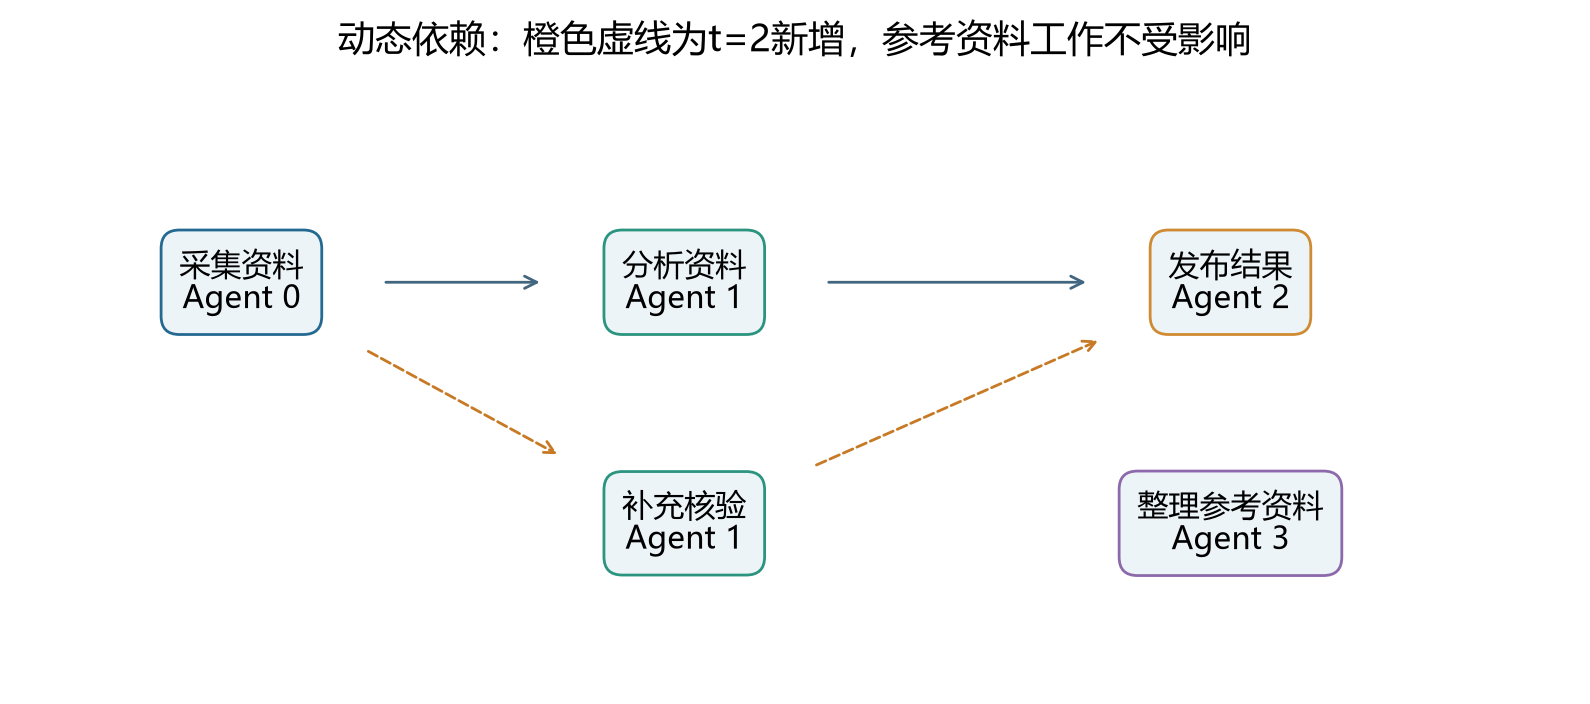
\includegraphics[width=0.85\textwidth,height=0.68\textheight,keepaspectratio]{../expr/015-tool-coordination/figures/dependency-change.png}
\caption{动态前置依赖变化：核验进入发布链，独立参考资料工作不受影响。}
\label{fig:dependency-change}
\end{figure}

新增核验条件后，需要修改的是交付链中相关成员的安排。局部法保持无关成员的计划版本为1，对照中该版本升至4、5，说明其反复安装方案；这不等于对照重复执行了工具工作。

\begin{figure}
\centering
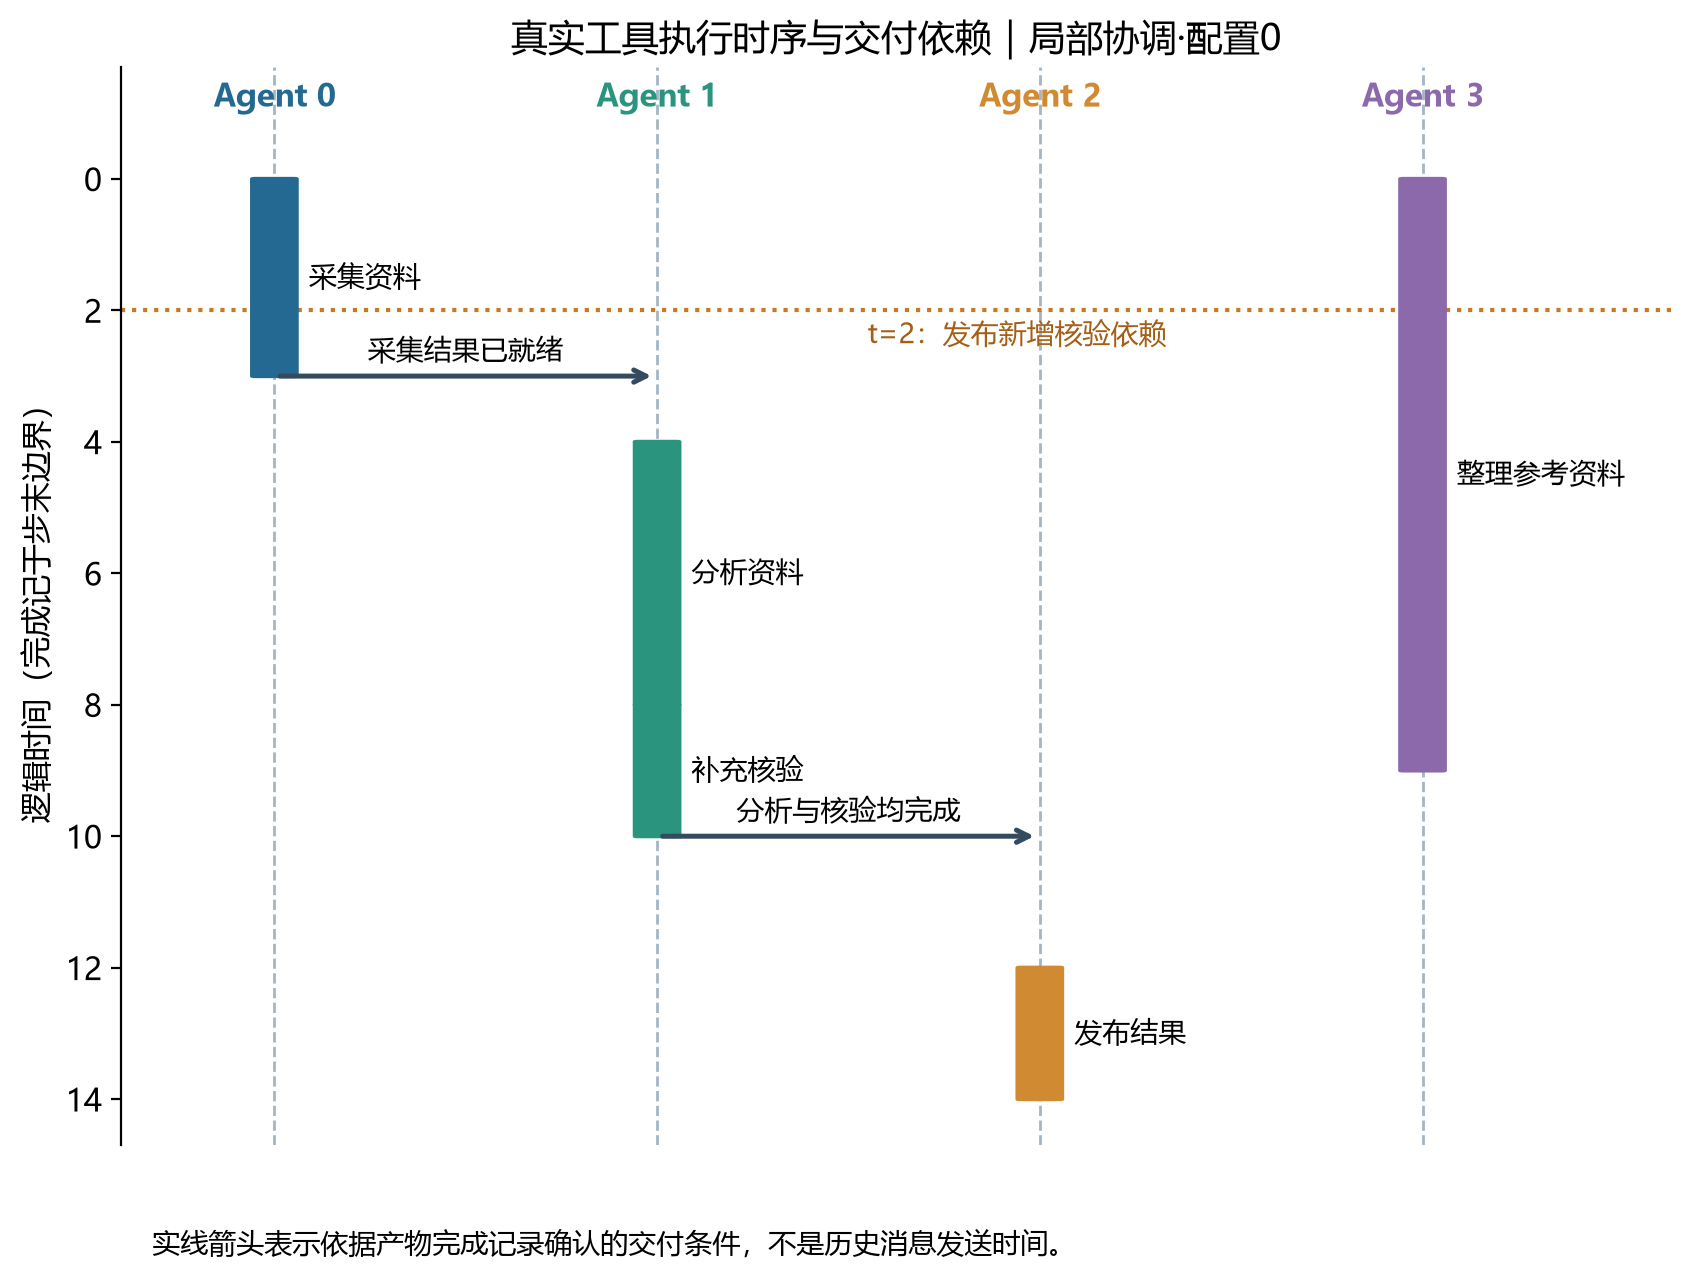
\includegraphics[width=0.9\textwidth,height=0.68\textheight,keepaspectratio]{../expr/015-tool-coordination/figures/execution-sequence.png}
\caption{工具执行时序：激活条来自真实工具记录，箭头表示前驱产物可用，不是精确的历史消息收发时间。}
\label{fig:execution-sequence}
\end{figure}

图\ref{fig:execution-sequence}展示了各成员的执行顺序：Agent0采集，Agent1分析并核验，Agent2等待前置交付后发布，Agent3独立工作。Agent2在分析与核验两项结果都到达后才开始发布。纵轴表示模拟逻辑时间。

\hypertarget{ux6309ux9700ux534fux8c03ux6210ux672c}{%
\section{按需协调成本}\label{ux6309ux9700ux534fux8c03ux6210ux672c}}

图\ref{fig:coordination-cost}比较了两个配置下的协调开销。模型调用合计为：局部法24次，全员重议45次，AutoGen适配36次；输入token分别为4268、8763、8398。相对AutoGen适配，局部法调用减少33.33\%，输入token减少49.18\%。

\begin{figure}
\centering
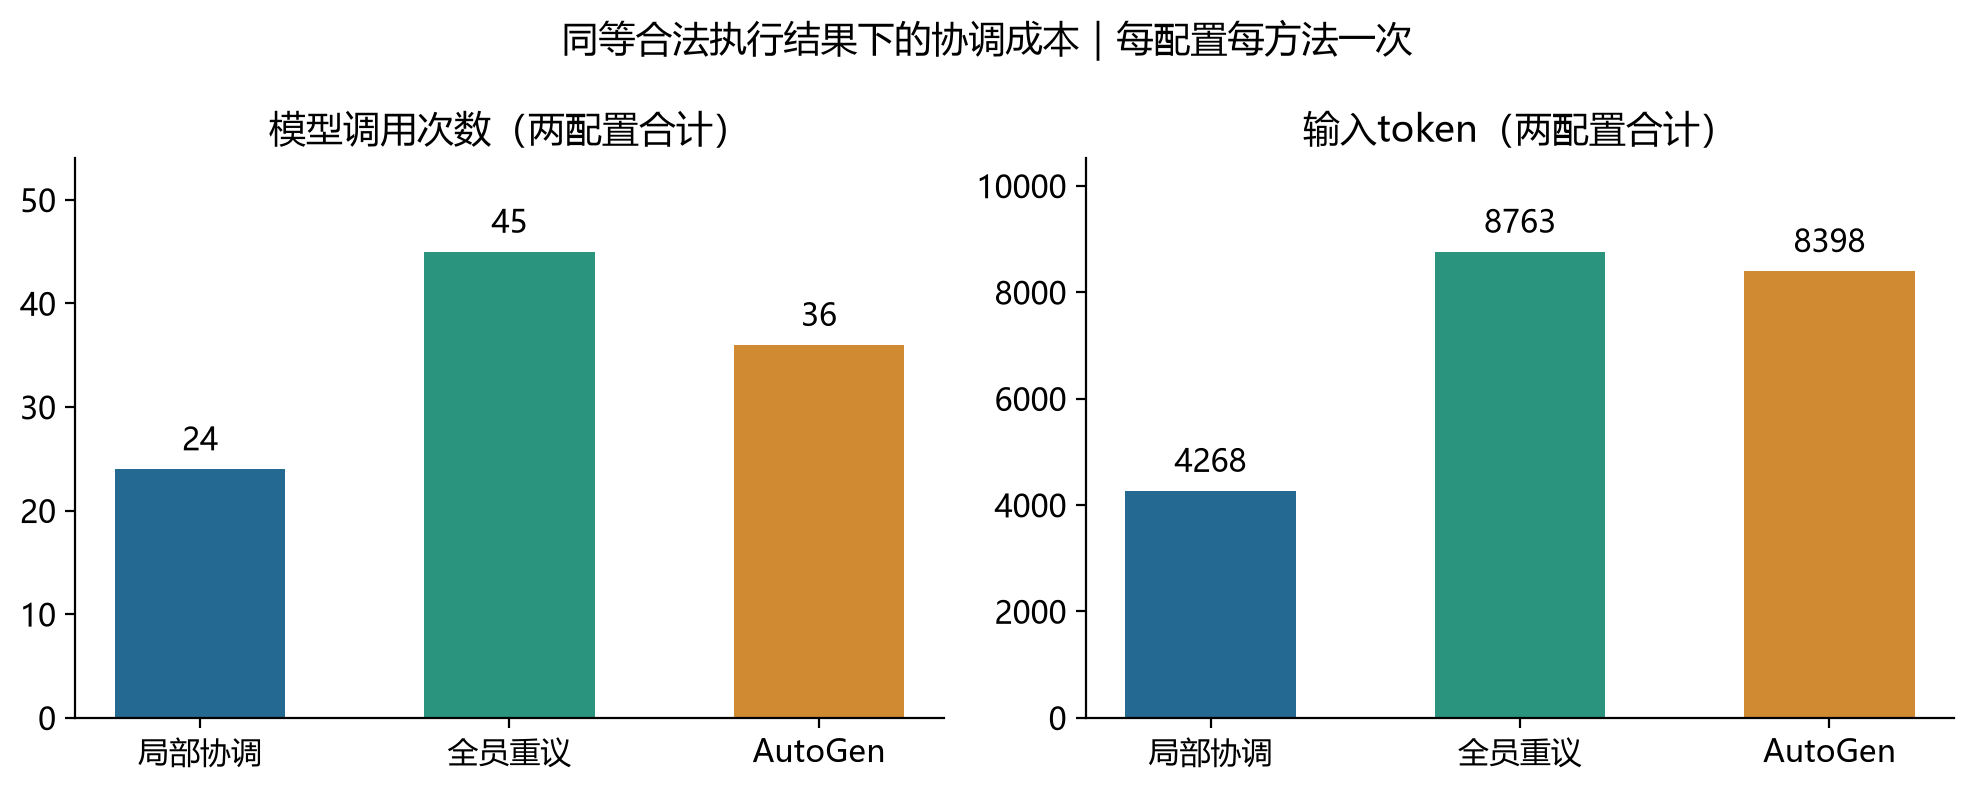
\includegraphics[width=0.85\textwidth,height=0.68\textheight,keepaspectratio]{../expr/015-tool-coordination/figures/coordination-cost.png}
\caption{同等执行轨迹下的协调成本，两配置各运行一次的合计。}
\label{fig:coordination-cost}
\end{figure}

在两个配置中，局部法与对照的执行轨迹相同，模型调用和输入token更少，节省主要来自减少重复协调。

\hypertarget{ux5916ux90e8ux4efbux52a1ux9a8cux6536marbleux66b4ux9732ux7684ux95eeux9898}{%
\chapter{总结}\label{ux5916ux90e8ux4efbux52a1ux9a8cux6536marbleux66b4ux9732ux7684ux95eeux9898}}

\section{工作总结与实验收获}

本作业从课程ReAct节拍的“再想”环节切入，形成了面向未来依赖的多Agent滚动协调设计。方法将任务工具与协调流程分离，由成员自行响应、相关方共同检查，并通过版本核验与局部安装保留有效安排。统一工具实验中，三种方法均完成任务；局部法在保持相同执行轨迹的同时减少了调用和输入开销，验证了按需协调的实际降本价值。

\hypertarget{ux7ed3ux8bbaux4e0eux5c40ux9650}{%
\section{实验局限与后续工作}\label{ux7ed3ux8bbaux4e0eux5c40ux9650}}

本作业围绕固定角色之后的多Agent协作，提出面向未来依赖的滚动协调设计，并实现相关方响应、局部更新和反馈触发机制。统一工具实验初步验证了依赖变化后的合法执行，以及复用有效安排减少模型调用的可行性。

\textbf{尚未证明的是：复杂任务中，跨Agent多步思考能够提高任务成功率。}
现有成本实验规模小、程序约束强；MARBLE验收则未形成有效协作。因而本文的结论是机制实现与初步验证，而非完整方法超越现有研究。

具体而言，任务所有者固定、多数合法动作域为单选，依赖变化由程序提供，尚未充分检验模型自主发现复杂依赖的能力。每配置仅运行一次，没有统计显著性；AutoGen对照包含每决策轮新建团队等适配选择，成本差异不能外推为框架普遍优劣。工具合法性也部分由程序约束保证，不能全部归因于模型规划。本作业尚需通过“各自多步规划”与“显式关联跨Agent依赖”的配对消融，进一步分离各机制的贡献。

后续先在一个已有协作任务上检查角色执行和任务结果，再使用相同模型、任务与预算，比较原生协作、各自多步规划和跨Agent依赖协调，记录成功率、通信、全部模型调用及耗时。
